\documentclass[aspectratio=169]{beamer}

\usepackage{ccicons}
\usepackage{fontspec}
\usepackage{listings}
\usepackage{tikz}
\usepackage{svg}

\definecolor{uclablue}{RGB}{39,116,174}
\definecolor{uclagold}{RGB}{255,179,0}

\definecolor{ubcorange}{RGB}{158, 66, 37}

\definecolor{cugold}{RGB}{207, 184, 124}
\definecolor{cudarkgray}{RGB}{86, 90, 92}

\definecolor{solarizedred}{RGB}{220, 50, 47}
\definecolor{solarizedblue}{RGB}{38, 139, 210}
\definecolor{solarizedgreen}{RGB}{133, 153, 0}
\definecolor{solarizedpurple}{RGB}{108, 113, 196}
\definecolor{solarizedmagenta}{RGB}{211, 54, 130}

\definecolor{pantone655}{RGB}{0, 42, 92}
\definecolor{pantone7453}{RGB}{123, 164, 217}
\definecolor{pantone633}{RGB}{0, 139, 176}
\definecolor{pantone7492}{RGB}{218, 229, 205}

\colorlet{primarycolor}{pantone655}
\colorlet{secondarycolor}{pantone7453}


\usetikzlibrary{
  arrows,
  arrows.meta,
  automata,
  backgrounds,
  calc,
  chains,
  decorations.pathreplacing,
  fit,
  intersections,
  matrix,
  overlay-beamer-styles,
  positioning,
  shapes,
  shapes.multipart,
  tikzmark,
}
\usetikzmarklibrary{listings}

\hypersetup{
  colorlinks=true,
  urlcolor=cudarkgray,
}

\setbeamercolor{frametitle}{fg=primarycolor}
\setbeamercolor{structure}{fg=primarycolor}
\setbeamercolor{enumerate item}{fg=black}
\setbeamercolor{itemize item}{fg=black}
\setbeamercolor{itemize subitem}{fg=black}

\setbeamersize{text margin left=26.6mm}
\addtolength{\headsep}{2mm}

\setbeamertemplate{navigation symbols}{}
\setbeamertemplate{headline}{}
\setbeamertemplate{footline}{}
\setbeamertemplate{itemize item}{\color{black}}
\setbeamertemplate{itemize items}[circle]

\setbeamertemplate{footline}{
  \begin{tikzpicture}[remember picture,
                      overlay,
                      shift={(current page.south west)}]
    \node [black!50, inner sep=2mm, anchor=south east]
          at (current page.south east) {\footnotesize \insertframenumber};
  \end{tikzpicture}
}

\setsansfont{Inter}[Scale=MatchLowercase]
\setmonofont{Hack}[Scale=MatchLowercase]

\makeatletter
\newcommand\version[1]{\renewcommand\@version{#1}}
\newcommand\@version{}
\def\insertversion{\@version}

\newcommand\lecturenumber[1]{\renewcommand\@lecturenumber{#1}}
\newcommand\@lecturenumber{}
\def\insertlecturenumber{\@lecturenumber}
\makeatother

\setbeamertemplate{title page}
{
  \begin{tikzpicture}[remember picture,
                      overlay,
                      shift={(current page.south west)},
                      background rectangle/.style={fill=pantone655},
                      show background rectangle]
    \node [anchor=west, align=left, inner sep=0, text=white]
          (lecturenumber) at (\paperwidth / 6, \paperheight * 3 / 4)
          {\Large Lecture \insertlecturenumber};
    \node [inner sep=0, align=left, text=white, node distance=0,
          above left=of lecturenumber, anchor=south west, yshift=2mm]
          {\Large ECE 344: Operating Systems};
    \node (title) [inner sep=0, anchor=west, align=left, text=white,
                   text width=30em]
          at (\paperwidth / 6, \paperheight / 2)
          {{\bfseries \Huge \inserttitle{}}};
    \node [inner sep=0, align=right, text=white, node distance=0,
          below right=of title, anchor=north east, yshift=-1mm]
          {{\footnotesize \ttfamily \insertversion}};
    \node [inner sep=0, text=white, align=left, anchor=west]
          (author) at (\paperwidth / 6, \paperheight / 4)
          {\insertauthor};
    \node [text=white, inner sep=0, align=left, node distance=0,
           below left=of author, anchor=north west, yshift=-2mm]
          {\insertdate};
    \node [align=right, anchor=south east, inner sep=2mm, text=white]
          (license) at (\paperwidth, 0)
          {\footnotesize This  work is licensed under a
           \href{http://creativecommons.org/licenses/by-sa/4.0/}
                {\color{pantone7453} Creative Commons Attribution-ShareAlike 4.0
                 International License}};
    \node [text=white, inner sep=0, align=right, node distance=0,
           above right=of license, anchor=south east, xshift=-2mm]
          {\Large \ccbysa};
  \end{tikzpicture}
}

\tikzset{
  >=Straight Barb[],
  shorten >=1pt,
  initial text=,
}

\lstset{
  basicstyle=\footnotesize\ttfamily,
  language=C,
  escapechar=@,
  commentstyle=\color{black!50},
}


\lecturenumber{29}
\title{SSDs and RAID}
\version{1.0.0}
\author{Jon Eyolfson}
\date{November 28, 2022}

\begin{document}
  \begin{frame}[plain, noframenumbering]
    \titlepage
  \end{frame}

  \begin{frame}{Solid State Drives (SSD) Are More Modern}

    Use transistors (like RAM) to store data rather than magnetic disks

    \vspace{2em}

    Pros

    \hspace{2em} No moving parts or physical limitations

    \hspace{2em} Higher throughput, and good random access

    \hspace{2em} More energy efficient

    \hspace{2em} Better space density

    \vspace{2em}

    Cons

    \hspace{2em} More expensive

    \hspace{2em} Lower endurance (number of writes)

    \hspace{2em} More complicated to write drivers for
  \end{frame}

  \begin{frame}{A SSD Contains Pages}
    \begin{center}
      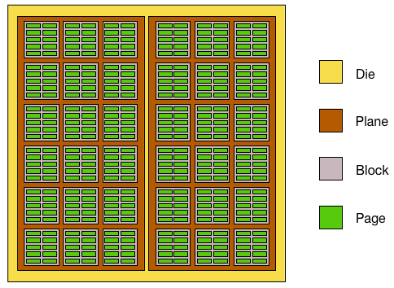
\includegraphics[height=0.8\textheight]{ssd.png}    
    \end{center}
  \end{frame}

  \begin{frame}{SSDs Using NAND Flash Are Much Faster Than HHDs}

    Pages are typically 4 KiB


    \vspace{2em}

    Reading a page: 10 μs

    Writing a page: 100 μs

    Erasing a block: 1 ms
  \end{frame}

  \begin{frame}{NAND Flash Programming Uses Pages and Blocks}

    You can only read complete pages and write to freshly erased pages

    \vspace{2em}

    Erasing is done per block (a block has 128 or 256 pages)

    \hspace{2em} An entire block needs to be erased before writing

    \vspace{2em}

    Writing is slow (may need to create a new block)
  \end{frame}

  \begin{frame}{The OS Can Help Speed Up SSDs}

    SSDs need to garbage collect blocks

    \hspace{2em} Move any pages that are still alive to a new block (may be overhead)

    \vspace{2em}

    The disk controller doesn't know what blocks are still alive

    \hspace{2em} SSD may think the disk is full, when a file could be deleted (not erased)

    \vspace{2em}

    The OS can use the \textit{TRIM} command to inform the SSD a block is unused

    \hspace{2em} The SSD can freely erase the block without moving overhead
  \end{frame}

  \begin{frame}{So Far We've Been Talking About Single Devices}

    Sometimes called Single Large Expensive Disk (SLED)

    \hspace{2em} Just one large disk for data

    \hspace{4em} Single point of failure

    \vspace{2em}

    There's also Redundant Array of Independent Disks (RAID)

    \hspace{2em} Data distributed on multiple disks

    \hspace{4em} Use redundancy to prevent data loss

    \hspace{4em} Use redundancy to increase throughput
  \end{frame}

  \begin{frame}{RAID 0 is Called a Striped Volume}

    Data stripes (128KB and 256KB) are distributed over disks

    \begin{center}
      \includesvg[height=5cm]{raid-0.svg}
    \end{center}
    
    \begin{flushright}
      by Cburnett licensed under CC BY-SA 3.0
    \end{flushright}
  \end{frame}

  \begin{frame}{RAID 0 is For Performance Only}

    The data is stripped across all disks in the array (you can have more than 2)

    \vspace{2em}

    Pro

    \hspace{2em} Faster parallel access, roughly $\mathsf{N}$ times speed

    \vspace{2em}

    Con

    \hspace{2em} Any disk failure results in a data loss (more points of failure)
  \end{frame}

  \begin{frame}{RAID 1 Mirrors All Data Across All Disks}

    \begin{center}
      \includesvg[height=5cm]{raid-1.svg}
    \end{center}

    \begin{flushright}
      by Cburnett licensed under CC BY-SA 3.0
    \end{flushright}
  \end{frame}

  \begin{frame}{RAID 1 is Simple, But Wasteful}

    Every disk in the array has a mirrored copy of all the data

    \vspace{2em}

    Pro

    \hspace{2em} Good reliability, as long as one disk remains, no data loss

    \hspace{2em} Good read performance

    \vspace{2em}

    Con

    \hspace{2em} High cost for redundancy (we can do better)

    \hspace{2em} Write performance is the same as a single disk
  \end{frame}

  \begin{frame}{RAID 4 Introduces Parity}

    Data stripes distributed over disks with a dedicated parity disk (p = parity)

    \hspace{2em} Parity stores xor $\oplus$ of copies 1-3, any one copy can be
                 reconstructed

    \begin{center}
      \includesvg[height=5cm]{raid-4.svg}
    \end{center}

    \begin{flushright}
      by Cburnett licensed under CC BY-SA 3.0
    \end{flushright}
  \end{frame}

  \begin{frame}{RAID 4 Can Use the Parity Drive to Recover}

    With parity, we can use $\mathsf{1 - \frac{1}{N}}$ of the available space

    \hspace{2em} Requires at least 3 drives

    \vspace{2em}

    Pro

    \hspace{2em} We get $\mathsf{(N - 1)}$ times performance
                 (removing parity disk)

    \hspace{2em} We can replace a failed disk and rebuild

    \vspace{2em}

    Con

    \hspace{2em} Write performance can suffer, every write must write to parity
                 disk
  \end{frame}

  \begin{frame}{RAID 5 Distributes Parity Across All Disks}

    Data stripes distributed over disks and each disk takes turns with parity
    blocks
    \begin{center}
      \includesvg[height=5cm]{raid-5.svg}
    \end{center}

    \begin{flushright}
      by Cburnett licensed under CC BY-SA 3.0
    \end{flushright}
  \end{frame}

  \begin{frame}{RAID 5 is an Improved Raid 4}

    It has all the same pros as RAID 4

    \vspace{2em}

    Write performance is improved, no longer a bottleneck on a single parity
    drive
  \end{frame}

  \begin{frame}{RAID 6 Adds Another Parity Block Per Stripe}
    \begin{center}
      \includesvg[height=5cm]{raid-6.svg}
    \end{center}

    \begin{flushright}
      by Cburnett licensed under CC BY-SA 3.0
    \end{flushright}
  \end{frame}

  \begin{frame}{RAID 6 Can Recover from 2 Simultaneous Drive Failures}

    Due to the extra parity, we can use $\mathsf{1 - \frac{2}{N}}$ of the available space

    \hspace{2em} Requires at least 4 drives

    \vspace{2em}

    Write performance is slightly less than RAID 5, due to another parity calculation
  \end{frame}

  \begin{frame}{There's More Options For Persistence}

    We explored two more topics: SSDs and RAID
    \begin{itemize}
      \item SSDs are more like RAM except accessed in pages and blocks
      \item SSDs also need to work with the OS for best performance (TRIM)
      \item Use RAID to tolerate failures and improve performance using multiple disks
    \end{itemize}
  \end{frame}

\end{document}
